\documentclass[mathserif]{beamer}
\usepackage{accents}
\usepackage{algorithm}
\usepackage{algorithmic}
\usepackage{amsmath}
\usepackage{booktabs}
\usepackage{color}
\usepackage{colortbl}
\usepackage{ifdraft}
\usepackage{mathrsfs}
\usepackage{mathtools}
\usepackage[normalem]{ulem}
\usepackage[labelformat=empty]{caption}
\usepackage[warn]{makecmds}
\usepackage{siunitx}
\usepackage{appendixnumberbeamer}
\mathtoolsset{showonlyrefs,showmanualtags}
\usetheme[secheader]{pecostalk}
\graphicspath{{figs/}}
\usepackage[sort&compress]{natbib}
\providecommand\newblock{} % DANGER, natbib/beamer incompatible
\renewcommand{\newblock}{} % DANGER, hack them to be compatible
% Custom commands used for notational purposes
%%%%%%%%%%%%%%%%%%%%%%%%%%%%%%%%%%%%%%%%%%%%%%

% Things which should behave like operators re: spacing
\DeclareMathOperator{\covariance}{Cov}
\DeclareMathOperator{\trace}{tr}
\DeclareMathOperator{\variance}{Var}

% Requires the `ifdraft' package be defined
\newcommand{\draftonly}[1]{\ifdraft{#1}{}}

% Source term from integral constraints
\newcommand{\Cs}{\ensuremath{\mathcal{C}}}

% Imaginary unit
\newcommand{\ii}{\ensuremath{\mathrm{i}}}

% Knudsen number with optional subscript
\newcommand{\Knudsen}[1][]{\ensuremath{\mbox{Kn}_{#1}}}

% Mach number with optional subscript
\newcommand{\Mach}[1][]{\ensuremath{\mbox{Ma}_{#1}}}

% Partial-something-by-partial-something-else derivatives
% Negative thin spaces added because Charter has too much space here
\newcommand{\pp}[2]{\frac{\partial\!{#1}}{\partial\!{#2}}}

% Prandtl number with optional subscript
\newcommand{\Prandtl}[1][]{\ensuremath{\mbox{Pr}_{#1}}}

% A reference value; a quantity less a reference value
\newcommand{\reference}[1]{\ensuremath{\left\{#1\right\}_{0}}}
\newcommand{\lessreference}[1]{\ensuremath{\left({#1}-\reference{#1}\right)}}

% Reynolds number with optional subscript
\newcommand{\Reynolds}[1][]{\ensuremath{\mbox{Re}_{#1}}}

% Source term from slow derivative
\newcommand{\Ssd}{\ensuremath{\mathcal{S}}}

% The symmetric part of a tensor
\newcommand{\symmetricpart}[1]{\ensuremath{\operatorname{sym}\left(#1\right)}}

% Denote something as a tensor
\newcommand{\tensor}[1]{\ensuremath{\accentset{\leftrightarrow}{#1}}}

% Take the transpose
\newcommand{\trans}[1]{{#1}^{\mathsf{T}}}

% The expectation operator
\newcommand{\expect}[1]{\operatorname{\mathbb{E}}\left[#1\right]}

% Victor's macros for notation
\newcommand{\fav}  [1] {\ensuremath{\widetilde{#1}}}  % Favre average
\newcommand{\fluc} [1] {\ensuremath{#1'}}             % Reynolds fluctuations
\newcommand{\ffluc}[1] {\ensuremath{#1''}}            % Favre fluctuations
\newcommand{\func} [2] {\ensuremath{#1 \! \left(#2\right)}}  % Function, IV
\newcommand{\mean} [1] {\ensuremath{\overline{#1}}}     % mean
           % Custom commands loaded from here

% http://tex.stackexchange.com/questions/110388
% I want 1e-2 not 1x10^{-2} from siunitx
\sisetup{output-exponent-marker=\ensuremath{\mathrm{e}}}

\setbeamertemplate{itemize/enumerate body begin}{\small}
\setbeamertemplate{itemize/enumerate subbody begin}{\footnotesize}

\makecommand{\z}{\phantom{0}}  % Facilitates column alignment
\makecommand{\Z}{\phantom{.0}} % Ditto
\makecommand{\n}{\phantom{$-$}}  % Ditto
\makecommand{\c}[1]{}          % Comment out material

\date{Nov. 8th, 2016}
\author[Nicholas Malaya]{Nicholas Malaya}
\institute{Department of Mechanical Engineering \\ The University of
Texas at Austin}
\title[Dissertation Defense]{%
    \mbox{Numerical Simulation of Synthetic,}
    \mbox{Buoyancy-Induced Columnar Vortices}
}

\begin{document}
%%%%%%%%%%%%%%%%%%%%%%%%%%%%%%%%%%%%%%%%%%%%%%%%%%%%%%%%%%%%%%%%%%%%%%%%%%%%%%

%===============================================================================
% Title page
\begin{frame}
%
\titlepage{}


%\begin{centering}
\mbox{{\scriptsize Acknowledgment: This material is based upon work
 supported}}
\mbox{{\scriptsize by the Department of Energy [ARPA-E] under Award
 Number [DE-FOA-0000670]}} 
%\end{centering}
\raisebox{-0.2in}{\hbox{
\includegraphics[width=4.5in]{figs/Footer}}\hfill}
%
\end{frame}

%===============================================================================



%%%%%%%%%%%%%%%%%%%%%%%%%%%%%%%%%%%%%%%%%%%%%%%%%%%%%%%%%%%%%%%%%%%%%%%%%%%%%%
% BONUS ROUND
%%%%%%%%%%%%%%%%%%%%%%%%%%%%%%%%%%%%%%%%%%%%%%%%%%%%%%%%%%%%%%%%%%%%%%%%%%%%%%
%
\appendix
\section{Extra Slides}

\begin{frame}
 \frametitle{Course list}
 \footnotesize
 \begin{table}[h]
  \centering
  \begin{tabular}{llll}
   \hline \hline
   Course \# & Semester & Course Name & Instructor \\ 
   \hline 
   ME381P   & 2014 Spr.   & Validation \& Uncertainty Quantification &
	       Prof. R.D. Moser \\
   ME 382R5 & 2014 Spr.   & Advanced Combustion & Prof. O.A. Ezekoye \\
   CSE 397  & 2014 Spr.   &  Comp. \& Var. Methods for
	   Inv. Problems & Prof. O. Ghattas \\
   SDS 384  & 2014 Fall   & Bayesian Statistical Methods & Prof. S.
	       Walker \\
   SDS 394  & 2014 Fall   & Scientific \& Technical Computing & Dr. V. Eijkhou \\
   ME 382P  & 2015 Fall   & Adv. Exp. Methods in Thermal/Fluids
	   & Prof. D. Bogard \\  
   \hline \hline
  \end{tabular} 
 \end{table}

\end{frame}

%
% mesh
%
\begin{frame}
 \frametitle{Mesh}
 
 \begin{figure}[htb]
  \centering
  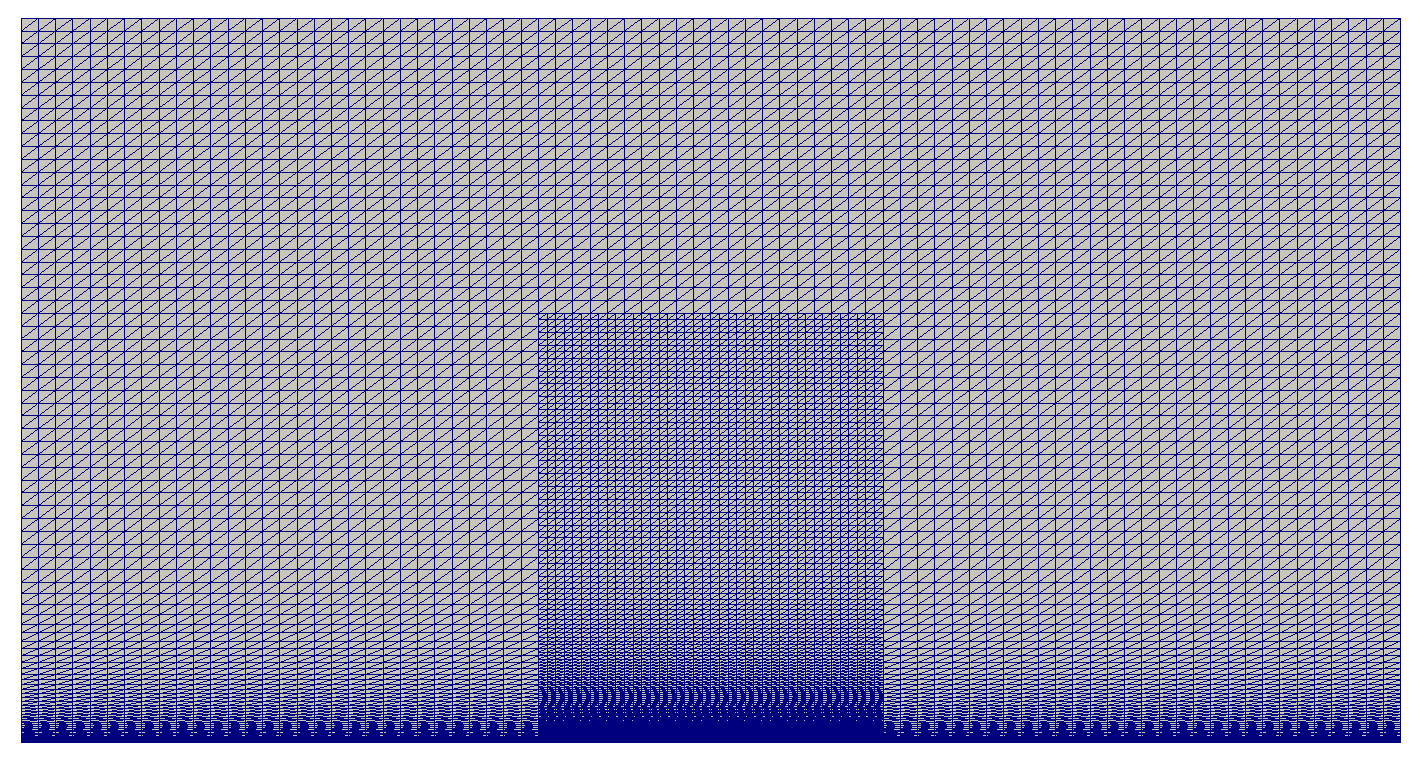
\includegraphics[width=.55\linewidth]{meshing}
 \end{figure}
 
 \begin{block}{Discretization}
  \begin{itemize}
   \item Single refinement in vane region
  \end{itemize}
\begin{equation*}
	  \text{Re}_\text{cell} = \frac{\text{max}(\Delta x,\Delta y)
	   \, u}{\nu_T}
\end{equation*}	
  \begin{itemize}
   \item Boundary layer mesh visible
  \end{itemize}
 \end{block}
\end{frame}

%
% SUPG Stab
%
\begin{frame}
\frametitle{Stabilization Outline}

\begin{itemize}
 \item Cast Navier Stokes + Boussinesq equations into weak form
 \item Prepare as operator $Lc=f$
 \item Calculate Fr\'echet derivative (to calculate operator adjoint)
 \item Separate into differential (P) and constant (Z) components,
       $L'[c] = P + Z$
 \item Choose stabilization operator such that $S = -P^*$
 \item Then stabilization has form, $a_h(c,\phi) = a(c,\phi) + \langle
       Lc,S\phi \rangle_\tau$
\end{itemize}


\end{frame}

\end{document}
